% geometry.tex -- Figure 1 of Chapter 3
% Kinematic geometry of a car with two off-hooked trailers.
% Standalone; \input it or \includegraphics the compiled PDF.
%
% The four lengths and three angles are the only symbols the rest of the
% thesis needs. Drawing proportions are exaggerated for legibility - say so
% in the caption.

\documentclass[tikz,border=8pt]{standalone}
\usepackage{amsmath}
\usetikzlibrary{arrows.meta,angles,quotes,calc}

% ---- pose used for the drawing (not the physical values) ----
\def\phideg{26}      % robot heading
\def\thAdeg{-9}      % trailer 1 heading
\def\thBdeg{-32}     % trailer 2 heading
% ---- lengths, drawing units ----
\def\dzero{1.45}
\def\lone{2.45}
\def\done{1.15}
\def\ltwo{2.45}
\def\halfw{0.80}     % half track
\def\wr{0.30}        % half wheel length

\newcommand{\axle}[3]{%   #1 = centre, #2 = heading in degrees, #3 = node name
  \coordinate (#3L) at ($(#1)+({\halfw*cos(#2+90)},{\halfw*sin(#2+90)})$);
  \coordinate (#3R) at ($(#1)+({\halfw*cos(#2-90)},{\halfw*sin(#2-90)})$);
  \draw[line width=0.8pt,black!70] (#3L) -- (#3R);
  \draw[line width=3.4pt,black!45,line cap=round]
        ($(#3L)+({\wr*cos(#2)},{\wr*sin(#2)})$) --
        ($(#3L)-({\wr*cos(#2)},{\wr*sin(#2)})$);
  \draw[line width=3.4pt,black!45,line cap=round]
        ($(#3R)+({\wr*cos(#2)},{\wr*sin(#2)})$) --
        ($(#3R)-({\wr*cos(#2)},{\wr*sin(#2)})$);
}

\begin{document}
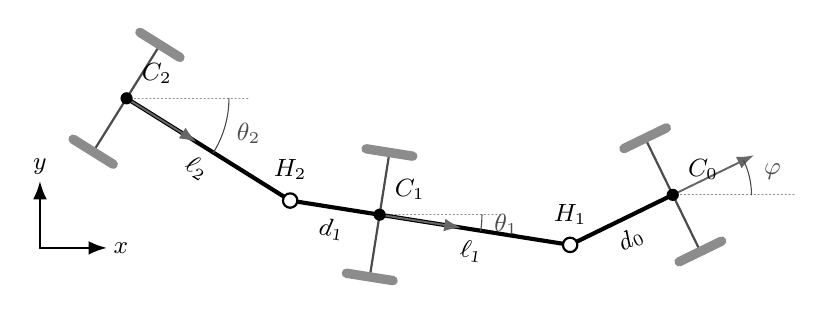
\begin{tikzpicture}[>=Latex,line cap=round,line join=round,
                    every node/.style={font=\small}]

% ================= the chain of points =================
\coordinate (C0) at (0,0);
\coordinate (H1) at ($(C0)+({-\dzero*cos(\phideg)},{-\dzero*sin(\phideg)})$);
\coordinate (C1) at ($(H1)+({-\lone*cos(\thAdeg)},{-\lone*sin(\thAdeg)})$);
\coordinate (H2) at ($(C1)+({-\done*cos(\thAdeg)},{-\done*sin(\thAdeg)})$);
\coordinate (C2) at ($(H2)+({-\ltwo*cos(\thBdeg)},{-\ltwo*sin(\thBdeg)})$);

% ================= horizontal references for the angles =================
\foreach \p in {C0,C1,C2}{
  \draw[densely dotted,black!45] (\p) -- ++(1.55,0);
}
\coordinate (R0) at ($(C0)+(1.5,0)$);
\coordinate (R1) at ($(C1)+(1.5,0)$);
\coordinate (R2) at ($(C2)+(1.5,0)$);

% heading directions (for the angle arcs)
\coordinate (F0) at ($(C0)+({1.5*cos(\phideg)},{1.5*sin(\phideg)})$);
\coordinate (F1) at ($(C1)+({1.5*cos(\thAdeg)},{1.5*sin(\thAdeg)})$);
\coordinate (F2) at ($(C2)+({1.5*cos(\thBdeg)},{1.5*sin(\thBdeg)})$);

% ================= bodies =================
\draw[line width=1.5pt] (C0) -- (H1);          % robot to first hitch
\draw[line width=1.5pt] (H1) -- (C1) -- (H2);  % trailer 1
\draw[line width=1.5pt] (H2) -- (C2);          % trailer 2

\axle{C0}{\phideg}{A}
\axle{C1}{\thAdeg}{B}
\axle{C2}{\thBdeg}{C}

% heading arrows
\draw[->,black!60,line width=0.7pt] (C0) -- ($(C0)+({1.15*cos(\phideg)},{1.15*sin(\phideg)})$);
\draw[->,black!60,line width=0.7pt] (C1) -- ($(C1)+({1.05*cos(\thAdeg)},{1.05*sin(\thAdeg)})$);
\draw[->,black!60,line width=0.7pt] (C2) -- ($(C2)+({1.05*cos(\thBdeg)},{1.05*sin(\thBdeg)})$);

% ================= hitch points and axle midpoints =================
\foreach \p/\lab/\pos in {C0/{$C_0$}/{above right}, C1/{$C_1$}/{above right}, C2/{$C_2$}/{above right}}{
  \fill (\p) circle (2.2pt);
  \node[\pos=2pt] at (\p) {\lab};
}
\foreach \p/\lab in {H1/{$H_1$}, H2/{$H_2$}}{
  \draw[fill=white,line width=0.8pt] (\p) circle (2.6pt);
  \node[above=4pt] at (\p) {\lab};
}

% ================= length labels =================
\path (C0) -- (H1) node[midway,below,sloped,inner sep=4pt] {$d_0$};
\path (H1) -- (C1) node[midway,below,sloped,inner sep=4pt] {$\ell_1$};
\path (C1) -- (H2) node[midway,below,sloped,inner sep=4pt] {$d_1$};
\path (H2) -- (C2) node[midway,below,sloped,inner sep=4pt] {$\ell_2$};

% ================= angles =================
\pic[draw,black!70,angle radius=10mm,angle eccentricity=1.30,"$\varphi$"]   {angle=R0--C0--F0};
\pic[draw,black!70,angle radius=13mm,angle eccentricity=1.24,"$\theta_1$"] {angle=F1--C1--R1};
\pic[draw,black!70,angle radius=13mm,angle eccentricity=1.24,"$\theta_2$"] {angle=F2--C2--R2};

% ================= world frame =================
\begin{scope}[shift={($(C2)+(-1.1,-1.9)$)}]
  \draw[->,line width=0.8pt] (0,0) -- (0.85,0) node[right,inner sep=2pt] {$x$};
  \draw[->,line width=0.8pt] (0,0) -- (0,0.85) node[above,inner sep=2pt] {$y$};
\end{scope}

\end{tikzpicture}
\end{document}
